
\documentclass{beamer}
\usepackage{changepage}
\usetheme{default}

\title{Git}

\author{Kiran Vasudev\inst{1}}

\institute[] 
{
  \inst{1}
  Hochschule Bonn-Rhein-Sieg

}

\begin{document}

\begin{frame}
  \titlepage
\end{frame}

\begin{frame}{Outline}
  \tableofcontents
\end{frame}

\begin{frame}[allowframebreaks]{Introduction}
\section{Introduction}
  \begin{itemize}
  \item {
    Most widely used Version Control System(VCS)
  }
  \item {
    Takes snapshots of the system.
  }
  \end{itemize}
\begin{figure}
	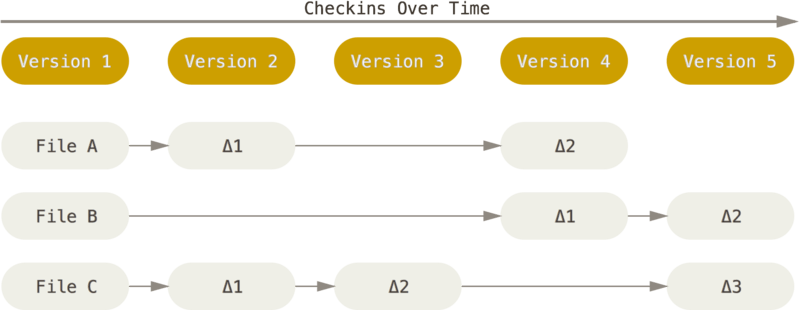
\includegraphics[scale=0.4]{images/deltas}
	\caption{Status of files in other VCS\cite{git-basics}}
\end{figure}
\begin{figure}
	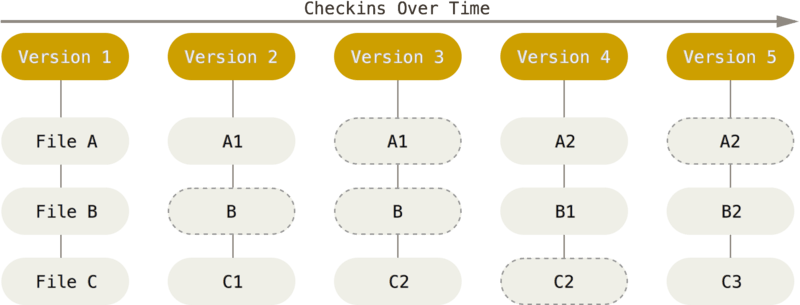
\includegraphics[scale=0.4]{images/git}
	\caption{Different versions in the form of snapshots\cite{git-basics}}
\end{figure}
\end{frame}

\begin{frame}{Main states of a Git repository}
\section{Main states of a Git repository}
  \begin{itemize}
  \item {
    Working directory
  }
  \item {   
    Staging Area
  }
  \item {   
    .git directory (repository)
  }
  \end{itemize}
	\begin{figure}
		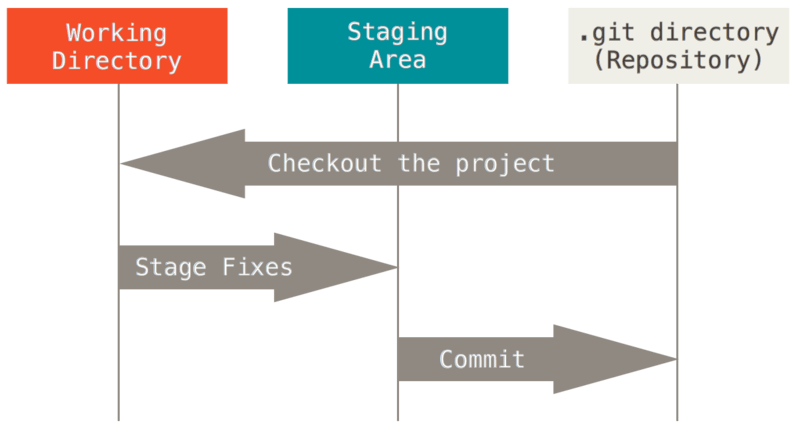
\includegraphics[scale=0.3]{images/areas}
		\caption{Working directory, staging area and the .git directory\cite{git-basics}}
	\end{figure}
\end{frame}

\begin{frame}{States of files in your working directory}
\section{States of files in your working directory}
	\begin{itemize}
		\item Files can either be tracked or untracked.
	\end{itemize}
	
	\begin{figure}
		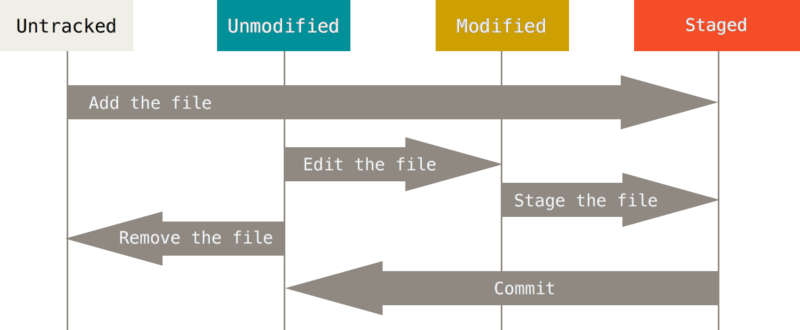
\includegraphics[scale=0.4]{images/lifecycle}
		\caption{Lifecycle of the status of files\cite{recording-changes-git}}
	\end{figure}
\end{frame}	

\begin{frame}[allowframebreaks]{Some important commands}
\section{Some important commands}
\textbf{Initializing}
	\begin{itemize}
		\item {\textbf{git config --global user.name "user-name"}}
		\item {\textbf{git config --global user.email "email-id"}}
		\item {\textbf{git init} \\ Initializes folder to be recognized as a git folder}
	\end{itemize}

	\textbf{Cloning}
	\begin{itemize}
	\item {\textbf{git clone} $\langle$remote\_location$\rangle$ $\langle$clone\_name$\rangle$ \\ Clones a repository into a new directory}
	\item {\textbf{git pull }$\langle$repository\_name$\rangle$\\Does a git fetch and then a merge}
	\item {\textbf{git fetch }$\langle$ target\_branch $\rangle$ \\Gathers commits from target branch and stores them in your local repository but does not merge them with the current branch }	
	\end{itemize}
	
	\framebreak
	\textbf{Tracking/removing files}
	\begin{itemize}
	\item {\textbf{git add} $\langle$f\_name$\rangle$\\ Adds the file to the stage}
	\item {\textbf{git rm} $\langle$f\_name$\rangle$\\ Removes the file from the working tree}
	\item {\textbf{git mv} $\langle$f\_name$\rangle$\\ Moves/renames the file in the working tree}
	\end{itemize}

	\textbf{Committing changes}
	\begin{itemize}
	\item {\textbf{git commit -m "message here"} \\ Commits the file to the repository} 
	\end{itemize}

	\textbf{Checking file status }
	\begin{itemize}
	\item {\textbf{git status} \\ To list out the status of files and folders}
	\item {\textbf{git diff} \\ Shows changes between commits}	
	\end{itemize}

	\textbf{Tagging }
	\begin{itemize}
	\item {\textbf{git tag} $\langle$tag\_name$\rangle$ \\ Used to tag a commit}
	\end{itemize}
	
	\textbf{Branching}
	\begin{itemize}
	\item {\textbf{git branch} \\ Lists the available branches. Can also be used to create a new branch with the argument $\langle$branch\_name$\rangle$}
	\item {\textbf{git checkout} $\langle$b\_name$\rangle$ \\ Switches to another branch}	
	\item {\textbf{git merge }$\langle$ b\_name $\rangle$ \\ Merges two development histories together}
	\end{itemize}

	\textbf{Viewing commit history }
	\begin{itemize}
		\item {\textbf{git log} \\ Lists the recent commit history}	
	\end{itemize}
	
	\framebreak
	\textbf{Working with remotes}
	\begin{itemize}
		\item {\textbf{git remote add} $\langle$remote\_name$\rangle$ $\langle$remote\_location$\rangle$ \\ Remotes are used to track repositories}
		\item {\textbf{git remote -v} \\ Lists all the remotes}
		\item {\textbf{git push} $\langle$remote\_name$\rangle$ $\langle$branch\_name$\rangle$\\Pushes local changes to the remote }
	\end{itemize}
	
\end{frame}	

\begin{frame}
	\begin{center}
		\Huge Lets get our hands dirty !
	\end{center}
\end{frame}

\begin{frame}{References}
  \section{References}
    
  \begin{thebibliography}{10}

  \bibitem{git-basics}
	\href{https://git-scm.com/book/en/v2/Getting-Started-Git-Basics}{Git basics}
	
  \bibitem{recording-changes-git}
	\href{https://git-scm.com/book/en/v2/Git-Basics-Recording-Changes-to-the-Repository}{Recording changes in Git}
	
	

  \end{thebibliography}
\end{frame}

\end{document}


